\documentclass{article}
\usepackage[utf8]{inputenc}
\usepackage{dirtytalk}
\usepackage{color}
\usepackage{tikz}
\usepackage[acronym]{glossaries}
\usepackage[backend=biber,style=authoryear,citestyle=authoryear]{biblatex}
\addbibresource{bib.bib}
\title{Responsibility Gap}
\author{Mischa}


\makeglossaries

\newacronym{mrinfes}{mRINFES}{Moral Responsibility is Important and Necessary for a Functional and Ethical Society}
\newacronym{cr}{CR}{Control Requirement}
\newacronym{ai}{AI}{Artificial Intelligence}
\newacronym{ml}{ML}{Machine Learning}
\newacronym{aws}{AWS}{Autonomous Weapon System}



%Numbered environment
\newcounter{example}
\newenvironment{example}[1][]{\refstepcounter{example}\par\medskip
   \noindent \textbf{Example~\theexample. #1} \rmfamily}{\medskip}


\begin{document}
\begin{titlepage}
	\maketitle
\end{titlepage}
\tableofcontents
\newpage
\section{Introduction}

This is a rough sketch of the beginning. It is very bad and not ready and I probably will
change most of it, but right now it kinda gives an introduction into the whole
topic.  

Nowadays it is an obivious statement to make that we live in a time in
which technology is ubiquitous and new technology is being developed at an
unprecidented rate. It penetrates our society and is one of the adhesives that
hold 'the system' in place. We must only envision a world in which cars do not
exist; or refrigerators; or the internet; or x-ray machines to see how much of
our (everyday) lives depends and is shaped by it. I also don't think that I go
out on a limb when I say that we integrate some technology relatively fast into
our lives. 

%Iphone in 2007 and a couple years later everybody has a smartphone
%bla bla bli blub

%Traffic lights are installed and programmed, perhaps superficially supervised
%and occasionally maintained and updated. peepee

In this work I will discuss technology and moral responsibility and how the two
relate to each other. Specifically, I will investigate the different ways we can seek
for moral responisbility in situations where an autonomous machine is involved.

Put more here.

But first, let us examine the traditional way of how we ascribe moral
responisbility in situations where technology is involved:

Suppose the following situations: A person hits another person with a hammer and
kills them. A newly installed dam breaks and a city is flooded. A hacker manages
to get access to a digital banking system through his own computer and steals a
good deal of money.\\

The hammer, the dam and the hacker's computer are technology that is directly
involved in morally critical situations. Yet, we abstain from blaming these
artifacts for what has happened in the respective situations. We also do not put
the events off as natural tragedies, as we do when a storm destroys a house or
an avalanche kills a skier in the mountains. We naturally ascribe the
responsibility for the events to the people behind the technology.
The person who wielded the hammer, the architect of the dam, the hacker.
These people used the technology as a tool to achive their own end and they are
responsible for the effects, that the technology has on our world, whether they
achieve the end or (as in the case of the dam-architect) not.
To view technology as tools or instruments used by humans and the humans as the ultimately
responsible entities for the technology is what Heidegger calls the \textit{instrumentalist
definition of technology} (\cite{heidegger1977technology}). 

\say{We ask the question concerning technology when we ask what it is. Everyone
knows the two statements that answer our question. One says: Technology is a means to an end. The
other says: Technology is a human
activity.}(\cite[p.4]{heidegger1977technology})

Thus, according to the instrumentalist definition, technology is something that
is intimately connected to humans and inherits its moral standing from the
quality of the \textit{human} end that it tries to achieve and from the way
it is used by \textit{humans}. Technology is not moral on its own. Only in the
context of human ends and actions. If it is humans that decide to use technlogy
for some end it is naturally them, who are responsible for the results.\\
A very similar line of reasoning is layed out by Sullins in what he calls the user, tool and victim
model (\cite[p. 152]{sullins2006robot}).

In the advent of machine learning we are facing a type of technology that is
intentinally becoming more and more autonomous, making decisions on its own
without any human supervision, without any human being able to predict or at
least explain those decisions. The Machines are essentially black boxes making
decisions and affecting the world in morally significant ways:

Autonomous Vehicles are being developed to populate the streets and naviagte
dangerous situations.
Machine Learning Algorithms analyse our behaviour on the internet, recommend
content that they find we would be interested in and influence us in this
manner.
There is a multitude of applications for ML in health care. We can easily
imagine that medical practitioners will increasingly rely on tools that diagnose
diseases and even propose treatments. Eventually, patients might even cut
out the middle man and receive their medical care from artificial physicians.
There already are services that provide a kind of psychotherapy by texting with
a chatbot. [zitieren]
Autonomous Weapon Systems (\acrshort{aws}) are being developed. The aim is to
create war robots that can be sent into the battle field and they would be able
to decide on their own whether to kill a target or not.

But what is the problem here? Why don't treat the vehicle, the recommender
algorithms, the health care systems, the war robots in just the same way as the
hammer, the dam or the computer from the examples above? Why not again hold the
operator or the manufacturer responsible? What is the difference? Why this
paper?


Include something like this:

Moreover, the situation makes us ask more fundamental questions: How do we
justify our practives of ascription of responsibility? What are morally
responsible agents. What are they responsible for? Depending on how we answer
these questions, results in different answers regarding the responsiblity gap
and how we deal with autonomous machines... bla bla bla



%Instrumental Theory:

%(\cite{johnson2006computer}): Computers are moral entites but not moral agents
%For most of the time human technology has been used as a tool.
%The user or manufacturer has the responisibility for what the tool does.
%This has been working so far quite well and the instrumental theory was a valid
%and accepted extension of our moral understanding.
%We are now in a time, where new technologies, that exhibit more and more
%autonomy challenge this stance, that they are mere tools. How should we handle
%des question of responisibility with this new technology? Is there are
%responisibility gap?
%
%Introduction of new technologies: ML

\subsection{The Dirty Problem}

The answer for these questions is the challenge that these technologies pose to
our traditional ways of ascribing responsibility.

According to Matthias (\cite{Matthias_2004}) the reason why we can hold either the
manufacturer or the operator of a machine responsible for what it effects in the
world, is because we can sensibly say that they are the moral agents who were in
control of said machine. Matthias claims that responsibility necessitates control:

\vspace{.8em}
\say{[An] agent can be considered responsible only if he knows the particular
facts surrounding his action, and if he is able to freely form a decision to
act, and to select one of a suitable set of available alternative actions based
on these facts.} (\cite[p.175]{Matthias_2004})

\vspace{.8em}
This means that we can only hold someone responsible for something they have
done, if they had sufficient control over their action.
This is widely referred to as the Control Requirement (\acrshort{cr}) [zitieren].

Converesly, if an agent does not have sufficient control, we can acsribe at most
partial responsibility, if any, to them.\\ 

This notion of control as a
precondition for responsibility seems to complement the intrumental theory: The
manufacturer and operator have control over their machines, thus they are the
ones who are responsible if something happens because of the machines. It is
then very clear how to assign responisbility in critical situations: If the
operator uses the machine in accordance with the manufactureres specifications
and something goes wrong, we say that the manufacturer is responsible. If the
operator deviates from the manufacturers specifications and something goes
wrong, we say the operator is responsible (\cite[p.175]{Matthias_2004}).

Enter Machine Learning:
We are now in a time where computer scientists and engineers work on increasing
the autonomy of their programs and machines by using techniques that can be
bundeled by the term \textit{machine learning} (\acrshort{ml}). `Autonomy' in this sense
means that we allow the technology to make its own decisions based on its
prior experience without the programmer or user knowing what the decision is
going to be or understanding how it came about.

%I WILL ALSO DEFINE AUTONOMY LATER. MAKE SURE THE TWI DEFINITIONS FIT TOGETHER OR
%POINt OUT THE DIFFERENCES OR WHATEVER

%Autonomie sich ziele zu setzen oder nur autonomie den weg zum vorgeggebenen ziel
%zu finden. 

%Put here: Machines can play Go, AWS, medical exper systems, even the youtube
%algorithm

This leads to a change in the classical roles of the manufacturer
(programmer) and operator (user) insofar that the amount of control they exert
over the machines diminishes as the machines become more and more autonomous.
Arguably, our traditional ways of ascribing responsibility are challenged. If we
agree with the CR and 

%Current practices in Artificial Intelligence (\acrshort{ai}) challenge this
%stance. The classical roles of manufacturer (programmer) and operator (user)
%change insofar that the amount of control they exert over the machines
%diminishes as the machines become increasingly autonomous.

%Current practices in Artificial Intelligence (\acrshort{ai}) aim at increasing
%the autonomy of machines and their software [zitieren]. `Autonomy' in this sense
%means that we allow the technology to make its own decisions based on its
%prior experience without the programmer or user knowing what the decision is
%going to be. In other words, they reduce the amount of control the programmer or
%user has over the machines. This is primarily the case for technology that uses
%machine learning to acquire a certain behaviour. [Passt hier eine beschreibung
%von machine learning rein?] At the same time the actions of
%such technologies have more and more impact on the people surrounding them
%[zitieren].\\

The real question:
Now here comes the question of this work: Who can sensibly be held responsible for the
actions of an autonomous machine?
Who is responsible if a driverless car runs over a person? Who is responsible if
an artificial physician proposes a wrong treatment for a patient? Who is
responisble for a war crime commited by an autonomous weapon system
(\acrshort{aws})?\footnote{Talk about asymetry of blame and reward. Refer to
later in next section perhaps, because here I mention responisbility only in the
sense of blaming someone}\\

Matthias says that our current practices of ascribing moral responsibility
fail at finding an appropriate target when an autonomous machine is
strongly involved in a situation. He calls this problem \textit{the
responsibility gap}.\\
%are not designed for dealing with autonomous machines and we are, thus, facing
%a responsibility gap. \\

The considerations above, do not entail that our current practices of
dealing with the effects machines have on our world must necessarily change,
but rather that the contemporary and foreseeable developments in AI and ML
challenge our current practices and motivate their reevaluation.

%WHAT THIS WORK IS NOT ABOUT: HOW CAN WE MAKE MACHINES THAT MAKE THE 'RIGHT'
%DECISIONS? HOW CAN WE MAKE MACHINES THAT MAKE ETHICAL CONSIDERATIONS ETC. THOUGH
%THERE IS A LOT OF OVERLAP THERE
%
%PUT SPARROWS CONCEPTUAL SPACE HERE. PERHAPS WITH A NICE GRAPHIC. Compare perhaps
%to Allan and Wallach diagramm of moral agency?


On the following pages I will first give descriptions of various accounts for
moral responsiblity and will then proceed to describing and debating the
different approaches philosophers have proposed for dealing with the assumed
responisbility gap.

%BIS HIER
%
%The idea that manufacturers and users lose control over an autonomous machine
%does not only stem from the theoretical definition of the word 'autonomous'. As
%Matthias argues, the loss of control can be found in the very way we put
%ML-techniques into practice (\cite[p.181-182]{Matthias_2004}). 
%
%Russell and Norvig define an agent as learning 
%
%\vspace{.8em}
%\say{if it improves its performance on future taskes after making observations
%about the real world.}(\cite[p.693]{russell2010artificial})
%
%\vspace{.8em}
%
%Technology that is being developed today often has the aim to become more and
%more autonomous. Autonomous in this sense means that we allow the technology to
%make its own decisions based on its prior experience without the programmer or
%user knowing what the decision is going to be. This is primarily the case for
%technology that uses machine learning to acquire a certain behaviour.
%As Matthias (\cite{Matthias_2004}) points out, the growing autonomy challenges our
%existing pracices for ascription of moral responsibility. Matthias says that
%in order to be responsible for something, one requires to be in control of it.
%This widely refered to as the Control Requirement (\acrshort{cr}) [zitieren].
%It follows, that neither the programmer, nor the user of an autonomous machine,
%can sensibly be said to be responsible for the actions of that machine.
%/newpage
\section{The Basics}

%TALK ABOUT THE SPLIT IN THE NOTIONS OF MACHINES AND RESPONSIBILITY BETWEEN
%AUTHORS.

Before jumping into any analysis of the responsibility gap as described above,
it makes sense to first explore what I mean, when I speak of the two things that
give this work its title. Moral responsibility and autonomous systems.
Additionally will draw attention to two different types of views bla bla.
\subsection{Two Perspectives}

%This part is very dirty. I don't think I will put it here, because it is too
%confusing for now. I will see, it it makes sense to include it somewhere else.



The process view and the property view.
I would like to introduce an idea by Daniel Tigard, that will serve as very
helpful tool to classify different approaches discribed in this piece. Though
Tigard relates that idea to specifically moral responsibility, I will try to
broaden its application. The pattern that is unveiled by that idea will follow
us throughout the following pages in different forms and variations, but it is
still unmistakable. When Tigard speaks of models of moral responsibility he
speaks that we may have a \textit{process view} or a \textit{property view} on
it CITATION. While I will examine what that means for moral responsibility with greater
detail later on
%DID YOU EXPLAIN IT MISCHA????
, I want to explain what these two possible views shall mean for us.

The two views are lenses that people use to explain some things we attribute to
each other. This seems like a very vague statement but allow me to elaborate:
What are these \say{things} that I mean? Well I mean stuff like consciousness,
moral responsibility, moral agency, intentionality, in short: all of those fine
concepts that philosophers hold so dearly by their hearts. From the property
view then, these things have some sort of metaphysical truth to them. The
subjects that we ascrive these things to, are said to have some kind of real
\textit{property} that gives rise to the thing and our perception of it. Without
this property on cannot truthfully say that the thing is there. Relating to
moral responsibility, Tigard says that \say{\textit{being} responsible [is]
conceptually prior to being \textit{held} responsible.}
To be rightfully held responsible, one must truly be responsible. To be
considered conscious, one mus truly by conscious. On the other hand, we have the
process view. The process view is another way of saying \say{It's a social
construct}. According to it, these things that we ascribe to ourselves and each
other are the results of a process of social and individual negotiation. The
thing is not born from some fundamental property, but from subjectively
\textit{being regarded as} existent. \say{\textit{[H]olding} is conceptually
prior to \textit{being} [...]}.

I understand if these two views lack any substance right now, but please bear
with me. Wou will lear to see them in what the people write. And with that we
shall continue.

%of two different views we can have on the
%things we will discuss in this piece.
%We can have the process view or we can property view on them. This idea stems
%from Daniel Tigard and he relates it to specifically moral resp
\subsection{What is Moral Responsibility}

While we generally have an intuitive understanding of what we mean
by (moral) responsibility, it is important for the following discussion to have
a more rigorous account of the term. The necessity of clarifiying the term
becomes clear, when we expose its ambiguity in our everyday language.
Sometimes we use moral responsibilty to say that someone has some sort of moral
obligation to do something. Sometimes we use the term to say that we blame
someone. Sometimes, to denote that a person is accountable for a certain action,
attitude or event in a sense that allows us to appraise them on its basis. And on and on...
%For one,
%holding someone responsible, often implies that they did something morally
%reprehensible. When we read or hear phrases like \say{I hold you responsible for
%	what you have done
%with the flowers.}, we often infer from that the speaker is blaming the person
%they are speaking with. However, most people would agree that being responsible
%for something does not imply blame. Being responsible can also mean that the
%person is praiseworthy. We can easily say that Florence Nightingale is
%responsible for founding modern nursing, something that people generally praise
%her for.

Angela Smith describes 3 different meanings that the sentence
\say{\textit{A} holds \textit{B} responsible for \textit{X}} can have:
(\cite[p. 469]{Smith_2007}):

\begin{enumerate}
	\item A thinks that B is open to moral appraisal because of X.\\
	\item A thinks that B is culpable and therefore blameworthy because of
		X.\\
	\item A blames B for X.
\end{enumerate}

For the sake of this work we are mostly interested in Smith's first sense of the
sentence. Thus, being responsible for something means that \textit{one is open to moral
appraisal for it}. In other words, when I am responsible for something, it means
that I am an appropriate target of blame, praise or other moral responses
because of it. PERHAPS THIS IS A GOOD MOMENT TO TALK ABOUT THE IMBALANCE IN R.
As we will see later, the same of very similar definitions of
responsibility can be found in other philosophical works on the topic. We
will, thus, continue working with it.

%This and similar definitions of responsibility can be found
%repeatedly in philosophical literature.

Now that we have agreed on what we mean when we speak of moral responsibility,
the questions that still remain are: What are the things that we are responsible
for? What are the conditions that need to be fulfilled to be morally responsible
for something (\cite[p. 370]{smith2008control})? Let us take a look at two
accounts that try to answer that question.


%NOTE: Criticise MATTHIAS FOR HIS CR. IT is not well defined. What is control. Control
%over future choices, past choices, what about situation where one does not have
%all the situation. Where does control end and so on.



%It is rather uncommon to use such phrasing to praise
%someone. In that sense the ord responsibility
%
%usually used in the context of blaming
%and far less often in the context of praising. Still, responsibility does not
%necessarily entail negative appraisal. We say that Marie Curie and and Henri
%Becquerel are responsible for discovering radioactivity and are generally
%praised for it. Angela Smith says that the phrase \say{A holds b responsible
%for X} can mean three different things:
%
%
%PUT SOMETHING HERE.
%ANGELA SMITH DESCRIBES THE DIFFERENT MEANINGS OF "A HOLDS B RESPONSIBLE FOR X"

\subsubsection{Strawson}

%There is an ongoing discussion in philosophy about the existence of determinism
%and its impact on free will, and some philosophers deem free will to be closely related to
%moral responsibility [zitieren]. To discuss this topic is notbla bla nor is it
%my intention to take a position on this issue. Instead I will try to elegantly
%sidestep the matter by taking a Strawsonian approach on moral responsibility.

%PERHAPS I CAN TAKE THAT FIRST PARAGRAPH OUT? NO NEED TO SPEAK OF DETERMINISM.
%
In ``Freedom and Resentment'' P.F.Strawson gives and account of our moral
practices and tries to explain the mechanisms behind them. These mechanisms lay
the groundwork for what can be understood as moral responsibility.
In the centre of Strawson's argumentation lies \say{the very great importance that
we attach to the attitudes and intetions towards us of other human beings
[...]}(\cite[p.5]{Strawson1962}). In other words, we care a lot about how other
people treat us. We like it, if other people treat us with what we interpret as
respect and goodwill and we do not like it, if other people treat us with what
we interpret as illwill or indifference. Depending on how other people treat us
and which attitudes we ascribe to them, we in turn develop and adjust our own
attitudes towards them. Strawson calls the attitudes we form as a reaction to
other people (quite fittingly) our \textit{reactive
attitudes}. Examples for such attitudes are resentment, indignation, gratitude.
These reactive attitudes form the basis for our practices of blaming and
praising other people.

%BEISPIEL EINFÜGEN!!


\begin{example}
	Matt is seventeen and likes playing computer games. His ten year old brother
	Charly often watches him play and frequently asks Matt, if he can play
	too. Matt usually denies Charly's request. Charly finds this unfair
	because Matt can play so much and he can only watch. Charly develops
	slight resentment against his brother because in his eyes, Matt
	does not care enough about him to fulfill Charly's wish of playing.
	Eventually, Charly runs to his mother and complains about Matt's
	unwillingness to allow Charly to play on the computer.
\end{example}

The primitive example above portrays the mechanism, Strawson tries to describe.
In the situation Charly interprets that his brother, Matt, treats him with an
attitude he does not like: indifference. This prompts Charly to develop
resentment towards Matt as a reactive attitude. Charly's going to his mother and
complaining about Matt is his way of blaming Matt.

Strawson stresses the importance of attitude behind an action, for we evaluate
other people and their actions strongly on the basis of their attitudes and
intentions. The same action with different attitudes elicits different reactions
from us. Strawson gives the example of someone stepping on his hand. If P-Boy
found that they did it accidentally and they were sorry for injuring him, he
would feel the pain in his hand, but probably no (appropriate) resentment
towards them. If, on the other hand, he found that they stepped on his hand out
of malevolence or were indifferent to what had happened, Strawsons reaction
would include some kind of resentment towards the other person. The same is
true, for when another person benefits us in some way. The degree of gratitude
we would feel towards them would differ, depending on whether they did it on
purpose and out of good will or accidentally (\cite[p.6]{Strawson1962}).


%Question for Uwe (perhaps): Is the person that steps on P-Boys hand not still
%responsible for doing so? They may not be open to appraisal, but it was still
%them, who did it. Is there an answer to that in Shoemaker? I don't think so.
%Perhaps some people would say that they were then causal

I should also point out, just like Strawson repeatedly does (\cite[p.5,
p.7]{Strawson1962}), that the way reactive attitudes work is much more
complicated than can be explained in this text. There is a complex
interplay between different parties and the attitudes vary on a broad spectrum
as well as in intensity.\\

The type of reactive attitudes I have described until now is generally about close
personal interactions with other people. They develop because of the way other
people treat specifically \textit{us}. 
However, reactive attitudes are not only a personal phenomenon but are also developed
and affected by how the objects of these attitudes treat other people.
Thus, Strawson introduces another class of reactive attitudes, which he calls
\textit{vicarious} or \textit{impersonal} reactive attitudes. These attitudes
target the behaviour or will of others independent of who is affected by them.
To be clear: These impersonal reactive attitudes can also be
developed if \textit{we} are the suffering party, but \say{[...] they are
essentially capable of being vicarious}(\cite[p.15]{Strawson1962})
%THE 'TO BE CLEAR' IS NOT AS CLEAR AS IT SHOULD BE.

Strawson proceeds and gives these vicarious reactive attitudes the
qualifier \textit{'moral'} and the objects of such reactive attitudes are said
to have done something that has moral value (positive or negative) to us
(\cite[p.15]{Strawson1962}). And thus, Strawson has linked the concept of
moralitiy with his reactive attitudes.


\begin{example}
	Clara likes to read the newspaper in the morning. Today, she finds an
	article about a CEO of a big international company and how he knowingly
	choses suppliers that violate human rights to drive the price of their
	commodities down. Clara does not like this behaviour.
\end{example}


It is clear that Clara is not personally affected (at least not directly) by the
behaviour of the CEO. She still develops a reactive attitude towards him on the
basis of his indifference regarding humabn rights and the people who suffer
because of it. What Clara experiences is moral indignation.

To sum it all up: According to Strawson, we expect from other people that they
behave in accordance with attitudes of respect and goodwill. Depending on
whether they cohere with these expectations, we exhibit resentment or gratitude
(reactive attitudes) towards them. We blame or praise other people on the basis
of these reactive attitudes. Morality comes into play, when we acknowlidge that
we expect certain behaviour not only towars us, \say{[...] but towards all those on
whose behalf moral indignation may be felt [...]} (\cite[p.16]{Strawson1962}).

In light of this account, moral responsibility does not seem to be a metaphysical entity.
From a Strawsonian perspective, to be morally responsible can be interpreted as
being an appropriate object of vicarious reactive attitudes
(\cite[p.3]{SmithVickers2021}) (\cite[p.175]{Matthias_2004}). Tigard takes moral
responsibility in this regard \say{as a social funtion of [...] reactive
attitudes} (\cite[p.3]{Tigard_2020}). 
These definitions cohere very well with the one I already mentioned above: To be
responsible means to be open to moral appraisal.

%HERE I MUST FINISH THE DIGRESSION AND EXPLAIN REFERENCE THE INITIAL QUESTION:
%WHAT ARE WE RESPONSIBLE FOR?

%FIND MORE INTERPRETATIONS AND PUT THEM
%INTO CONTEXT

%SHOEMAKER SAYS: MORAL RESPONSIBILITY IS, AT LEAST IN PART, BEING OPEN TO A
%CERATAIN RANGE OF MORAL RESPONSES (PAGE 11)


Before moving on, Strawson, introduces another idea, which might be important for
our further discussion on the main topic of this work, the responsibility gap.
He describes in which cases reactive attitudes are mitigated or even not
exhibited at all. Strawson distinguishes two general groups of such cases:

\begin{enumerate}
	\item Cases of the first group are those where the source of injury is a
		moral agent but their explanation for their action can be
		summarised with the sentences `I didn't know', `I had to do it'
		or something similar (\cite[p.7-8]{Strawson1962}). Tigard
		descibes these cases as situations \say{where the agent is
		normal, but the circumstances are abnormal [...]} 
		(\cite[p.5]{Tigard_2020}).

		Examples of such cases are the gentleman who accidentally steps
		on someones foot because the train is too full and he tries to
		navigate through the crowd, or the doctor who has lost a patient
		and is then rude to her husband. The people who suffer the
		injury usually tend to modify their reactive attitudes to fit
		the circumstances.
		TIGARD HAS A SIMILAR EXAMPLE



	\item The second group is again nicely described by Tigard as cases
		\say{where the circumstances are normal but the agent is
		abnormal} (\cite[p.5]{Tigard_2020}). Strawson speaks of children
		or schizophrenics or people that act out of compulsion
		(\cite[p.8-9]{Strawson1962}). Such
		agents cannot be appropriate targets of reactive attitudes
		because the expectations upon which the reactive attitudes are
		based cannot be reasonably targeted towards them. According to
		Strawson, it is unreasonable to expect moral behaviour from
		someone who is morally deranged or underdeveloped. In this
		sense, they are not moral agents and cannot be treated as such.
		We do not see them as members of the moral community
		(\cite[p.18]{Strawson1962}). The attitudes we exhibit towards
		them differ accordingly compared to those who are members of the
		moral community. We see them as \say{object[s] of social policy;
			as [...] subject[s] for [...] treatment; as something
			certainly to be taken account, perhaps precautionary
			account, of; to be managed or handled or cured or
		trained; perhaps simply to be avoided [...]}
		(\cite[p.8]{Strawson1962}). Seeing an agent as such, implies
		that we portray a second set of attitudes towards them. Strawson
		calls these attitudes \textit{objective attitudes}
		(\cite[p.9]{Strawson1962}). 
\end{enumerate}

I want to reiterate: To have reactive attitudes towards someone \textit{means}
to view them as a fully responsible agent. In Strawson's eyes these are the same
things (\cite[p.23]{Strawson1962}). To have objective attitudes towards someone (or something)
\textit{means} to view them outside of the moral community and, thus, to view
them as an inadequate target for ascribing responsibility. \#foreshadowing\\
\textit{It means that only full moral agents (members of the moral community) can be
morally responsible for their actions}.  This is a very important insight that
will become relevant later on.
\label{responsibility_implies_agency}

%STRAWSONS ACCOUNT DISMISSES THE METAPHYSICAL VALUE OF MR. INSTEAD IT IS
%SUGGESTED THAT MR HAS ONLY SOCIAL AND PSYCHOLOGICAL SIGNIFICANCE

%UNDER STRAWSONS ACCOUNT THERE IS NO SUCH THING AS MORAL RESPONSIBILITY. THERE IS
%ONLY THE SOCIAL NEGOTIATION OF INTERPERSONAL ATTITUDES IN A SOMEWHAT DIALECTIC
%MANNER. THERE IS ONLY CAUSAL RESPONSIBLITY AND THE REACTIVE ATTITUDES ATTATCHED
%TO IT. (HOLDING RESPONSIBLE)
%AT THIS POINT IT IS A QUESTION THAT WE SHOULD ASK IN A MORE SOCIOLOGICAL AND
%PSYCHOLOGICAL SETTING RATHER THAN A PHILOSOPHICAL ONE.

\subsubsection{Smith}
\label{smith}

I already have repeadetly used such phrasings as `inadequate target' or
`appropriate object' of moral responsibility or reactive attitudes or blame or
praise. However, the attentive reader will find that Strawson's account of our
moral practices focuses strongly on our external perceptions of other's
internal attitudes.

In this regard, we are prone to say, that someone is an
appropriate object of, for example, blame, if (1) we see them as a member of the moral
community (we can develop reactive attitudes towards them) and (2) we
\textit{interpret} their attitudes as malevolent or indifferent towards us. But what
about the cases where our interpretation is wrong? We might think their action
is an expression of ill will towards us, but by looking beneath their sculp, we
might see that it is actually not the case and we had misinterpreted their
attitude. Intuitively, it would not be fair to blame someone, if their
\textit{actual}
attitude would not correspond with our \textit{perception} of their attitude.
Or their action was subject to circumstances unbeknownst to us. We hold them
responsible and blame them for the action. But upon learning more about the
circumstances we change our mind and judge the person to be not responsible
anymore. In fact, we say that they have not been responsible at all even for the
time we thought they were responsible. Does this not show that there is a sense
of being responsible that goes beyond `being held responsible' by others? Does
this not show that we in general do believe in a kind of responsibility relies
less on our perception and more on the truth of the situation? 
Smith argues that there is a difference in being held responsible and 
\textit{being} responsible. And it would not be fair for us to hold someone
responsible, if they `in reality' are not responsible (\cite[p.
472]{Smith_2007}).\\




% \textit{Oh hey what is that? I think that is determinism creeping in the
%	 background! Oh no, I hope nobody will notice it! *MISCHA USES HIS
% SPECIAL ATTACK: \textbf{GLOSSING OVER STUFF THAT MIGHT BE VERY IMPORTANT}*}\\
%
% \textit{Can you feel its presence? It is still at distance, yet comes closer the more we
% seek for truth. It regards us patiently as it is the end boss and it waits for
% a fight that may never halt. And the fight might never halt; not because we are
% equal adversaries, but because we are too weak to know when it is over.}
%
% \textit{It's breath is cold and merciless. It knows. But as the great minds, whose work
% is the basis of the words you read, I shall continue to ignore this final
% question and move on. And I ask the same of you. With the words of the russian
% writer Mikhail Bulgakov: Follow me, reader!}

%TAKE OUT THIS NEXT PARAGRAPH. IT IS TOO SPECULATIVE. WHAT ABOUT THE WHOLE
%THING FROM BEFORE? i MIGHT CHANGE THE WHOLE SECTION, TO BE MORE GENERAL ABOUT
%PROPERTY VIEW RESPONSIBILITY. THEN I CAN INCLUDE SHOEMAKER AND SCANLON AND NOT
%GO IN SO MUCH DETAIL.
%I believe, Strawson would answer to this, that his account of our moral practices
%does not claim to be fair or fulfill all the demands we might have towards said
%practices. Nor is it necessarily internally consistent. In this sense, it is
%not normative but largely descriptive. In practice, when blaming someone, we do
%not distinguish between our percetion of their attitude and their \textit{real}
%one. I suspect, that even if Strawson would acknowledge the differnce
%between being held responsible and being responsible, he would say that the
%latter notion has no practical relevance in our moral practices.

We can take Strawsons account of responsibility as a description for when
people are \textit{held} responsible in Smiths sense. But how can we make sense
of people \textit{being} responsible?\\

There are two opposing stances on that. Unified approaches vs pluralistic
approaches. Unified approaches are...
Pluralistic approaches are ...

I will briefly present Smiths unified apporach of moral responsibility in order
to get a sense of what I generally mean by people being responsible. Still, we
shall not forget, that this is only one of many accounts of moral responsibility
of there.

But how does Smith then
make sense people \textit{being} responsible? She proposes an approach, which
she calls the rational relations view CITE.

According to Smith, to be responsible for an action, attitude or mental state,
one must have a specific connection to it
%we hold people responsible for actions, attitudes and
%mental states that they have a specific type of connection to 
(\cite[p 370]{smith2008control}). What is this connection? The connection
cannot be that the action, attitude or mental state is attributable to me. I am
not responsible for feeling hungry, a person with epilepsy is not responsible
for having seizures, even though these are a things that can
properly be attributed to me and Epilepsy-Eric (\cite[p.
584]{smith2012attributability}). Thus, we are not responsible for everything
that is attributable to us. One might now come up with the idea that we are
responsible for our conscious choices, but Smith argues that the condition of
volition does not satisfyingly cover the domain of responsibility. We might be
responsible for actions and attitudes we deliberatly choose to take or have,
but in general we can also be responsible for actions and attitudes that are
not deliberate but spontaneous and involuntary. An example that Smith brings up
is her forgetting her friends birthday. She did not choose to forget the
birthday, she did not undergo a thought process that weighed the pros and cons
of forgetting the birthday and then arrived at the conclusion that it would
make sense to ignore the birthday. It just happened. She called her friend as
soon as she remembered congratulated her and apologised for forgetting. Of
course her friend forgave her but the implicite assumption still was that
Smith was responsible for forgetting the birthday. In general, people are also
considered responsible for their emotional reactions and arguably these are not
subject to deliberate choice. One could argue now that, if not choice, control
is what makes someone respnsible. And by control I mean that a person has the
theoretical control over the things they are doing, perhaps through past
choices, perhaps through the ability to change a certain aspect of oneself in
the future. After all, Smith had the control to write down her friends birthday
in her calendar and install a reminder and she has the control over making sure
that such a thing will not happen again. This sounds very similar to Matthias' control
requirement (\cite[p.175]{Matthias_2004}) that we have already introduced in
the first section. For Smith, this account, though plausible, is not satisfying
(\cite[p. 251]{smith2005responsibility}). Because what we find bad is not the
fact that Smith did not take any measures to be reminded of her friends birthday,
but rather that her forgetting her friends birthday shows (on the surface) that
Smith does not value her friend enough to remember it. The assumption is that
if Smith had judged the friendship to be important enough, she would have had
thought of that significant date.

% PERHAPS IT IS A GOOD IDEA TO PUT THIS IN AND EXPLAIN WHY SHE THINKS THAT
% Smith says that \say{[w]hen we praise
%	 or criticize someone for an attitude it seems we are responding to
% something about the content of that attitude and not to facts about its origin
% in a person's prior voluntary choices, or to facts about its susceptibility to
% influence though a person's future voluntary choices.} (\cite[p.
% 251]{smith2005responsibility}). An account of responsiblility that only relies
% on control 
%
% That control may be a common factor among
% the actions and attitudes we are responsible for, does not go to the heart of
% our moral practices. 

These kinds of judgements are the basis of Smith's rational relations view.
% THE TRANSITION DOES NOT WORK ANYMORE
%Instead Smith proposes that we are responsible for those things, for which it
%is reasonable to ask us to defend ourselves, or, to use Smith's words, for
%which we are answerable (\cite[p. 251]{smith2005responsibility}). 
Let us examine how she develops her idea.

According to Smith, people make certain judgements of \say{value, importance,
or significance} (\cite[p. 251]{smith2005responsibility}). These
\textit{evaluative judgements} can be abstract and form individual normative
ideals, like valuing freedom more than security, or they can be more concrete
like judging spiders to be dangerous. The judgements people make should
\textit{rationally}\footnote{I find that Smith uses the word
	 \say{rational} in a very loose sense. She probably does not mean
	 rational in the idealised and logical way, but rather in a more
	 holisitc sense. If my interpretation is correct the word
\say{reason-giving} as it is used by Shoemaker is a bit more
fitting (\cite[p. 23]{Shoemaker_2011}).} lead to certain behaviour in accordance with the
judgements (\cite[p. 244, p. 247, p. 250]{smith2005responsibility}). Thus, the
attitudes and actions are a direct reflection of evaluative judgements. Smith
argues, if a persons behaviour is based on such an
evaluative judgement, they are \say{open, in principle, to demands for
justification} for their behaviour (\cite[p.
577-578]{smith2012attributability}). This is what she calls
\textit{answerability}. So, people are answerable for their behaviour, if they
are theoretically able to reference a judgement that the behaviour was
expressing and to defend and justify that judgement. Further,
she states that moral appraisal of an agent \say{always embodies (at least implicitly) a
demand to her to justify herself} (\cite[p. 578]{smith2012attributability}).

Let us now connect all the dots: Being responsible is being open for moral
appraisal. Moral appraisal \textit{always} encompasses demands of justification. Such
demands only make sense, if a person is answerable for the appraised action or
attitude, meaning \say{that the thing in question must in some way reflect [the
persons] judgement or assessent of reasons} (\cite[p.
103]{smith2015responsibility}). According to Smith, people are responsible for
all and only those things, for which they are also answerable (\cite[p. 251,
p.256]{smith2005responsibility}).



% The people can then be asked to justify their behaviour and they
% can answer with a reference to and a justification of their judgement. Smith
% says that the people are \textit{answerable} for their behaviour, if 


An important property of these
\textit{evaluative judgements} is, that they must not \textit{necessarily} be
on the conscious radar or arrived at though deliberate thought. They can also
be sponataneous judgements that the person only forms or discovers when being
confronted with a new situation (\cite[p. 251-252]{smith2005responsibility}).

\begin{example}
	 Melissa has never thought much about her becoming a victim of sexual
	 assult. It is not a topic that crosses her mind in general. One night
	 she walks home through a dark alley and she spots a man walking
	 behind her. To her own surprise, she finds herself being afraid of that
	 man. The fear makes Melissa walk faster with the hope of getting more
	 distance between her and the man and getting home faster.
\end{example}

In the example, we see Melissa discovering her judgement that a man can
be potentially dangerous to her. The judgement arises sponatneously without her
having thought much about forming it and it elicits certain attitudes
and actions in Melissa. She experiences fear and walks faster because of it.
Notice also that Melissa's judgement is open to critical assessment; As soon as
she is aware of her judgement she has the possibility to think about the
judgement and decide whether it is justified or not.
Now, according to Smith, there is a rational relation between Melissa's
judgement and her attitudes and actions. Melissa's actions and attitudes are
expressions and reflections of her judgements. Melissa can thus justify her behaviour
by referencing and defending the evaluative judgements that caused it. She is
answerable for her behaviour. And that is what makes her responsible for it.

% So when Smith says that a person is answerable for something, she means that
% the person is in some way expressing an evaluative judgement and it is
% reasonable to ask them to rationally\footnote{I find that Smith uses the word
%	 \say{rational} in a very loose sense. She probably does not mean
%	 rational in the idealised and logical way, but rather in a more
%	 holisitc sense. If my interpretation is correct the word
% \say{reason-giving} as it is used by Shoemaker is a bit more
% fitting (\cite[p. 23]{Shoemaker_2011}).} defend that judgement. The defence is
% then the basis for their appraisal. And, on Smith'S account, people are
% responsible for all and only those things, for which they are answerable.

To summarise:
When we think that someone is morally responsible for something, we
\textit{might} demand a justification for their conduct before we
appraise them. The assumption is that their conduct is a direct result of their
explicit or implicit judgement. Our appraisal is then formed on the basis of
their justification for their judgement or, in other words, their answer to our
demand. If it is reasonable to make such a demand for justification the person
is said to be answerable. And according to Smith, people are responsible (open
to moral appraisal) for all and only those things they are answerable for.

% Some of the actions we take and the attitudes we adopt are rooted in
% judgements
% about the world, other people and ourselves. They can be judgements of
% prefence, value, significance and belief. They can be the result of
% deliberate thinking, but they might also arise spontaneously. Such judgements
% can be critically assessed by their holder as well as by other moral agents.
% Because of that, we can say that 
%
% These judgements express themselves in our actions and attitudes.
%
%
%
% answerability is just the condition for responsibility.
%
% This is what Smith means when she talks about \textit{answerability}. 
% Being responsible for an action or attitude, on Smith's account, is 
% being answerable for the underlying evaluative judgement. Further, we are
% responsible for all and only those actions and attitudes that can reasonably
% said to have an evaluative judgement as a basis for them. This rules out being
% responsible for having hunger or seizures.
% One is
% answerable for their actions and attitudes, if they are grounded in an
% evaluative judgement that rationally should elicit them.
%
%
% Actions, attitudes and mental states that
% express such evaluative judgements are exactly what we are responsible for.
%


% We will now look at an account of
% responsibility, that tries to explain when people \textit{are} responsible.
%
% If Smith 
%
% THIS IS SOMETHING THAT I WANT TO SAY, BUT BETTER: I ACTUALLY NOW THINk, THAT I
% DON'T NEED IT.
% Being a descriptive account of our moral practices, we can take it as it is
% standing alone, but it is also capable of leaving enough space to place a
% normative theory inside of it to complement and it. Shoemakers account of
% responsibility is such a theory, that can be placed into strawsons account.
%
% Angela Smith mentions the difference between being held responsible and being
% actually responsible
%
% Still, we find other philosophers seeking for a more rigorous and satisfying
% account of `appropriate' in this context. We have encountered one such approach
% in Matthias' control requirement (\cite[p.175]{Matthias_2004}), which we will
% dicuss in a later section. @FUTURE\_MISCHA: HAVE YOU REALLY DISCUSSED IT? DO
% YOU HAVE ENOUGH MATERIAL TO DISCUSS IT?
%
% CR REFERS TO ANSWERABILITY ACCORDING TO SHOEMAKER! HOW ABOUT THIS{
%	 Do you remember Matthias Control Requirement, that I have introduced in
%	 section 1.1? Well it bascally means bli bla. This kind of
%	 responsibility refers to answeability responsibility as Shoemaker calls
%	 it. But Shoemaker also states that it is not the only kind of
%	 responsibility. He provides two more types: Bla bla blib
%
% I also want to introduce an additional approach, proposed by David Shoemaker
% (\cite{Shoemaker_2011}). DA SHOE tries to give an account of what it means to
% be truly responsible. He proposes three distinct types of responsibility:
% Answerability, Attributability and Accountability.
%
% By Answerability Shoemaker means that people are responsible (i.e. open for moral
% appraisal) for the reasons they take to justify their actions. Let us remember
% the CEO from example 2. Suppose, when he was deciding which supplier to buy the
% commodities from, he did engage in a process of deliberate thinking and came to
% the conclusion that it was better to buy from 
%
% Fro mthis it is easy to interpret that moral responsibility
% rests solely on other's impression of one's will (though this is not a
% necessary conclusion or even something that Strawson argues for). In this regard, we might
% want to say that this seems too one-sided. If Strawsons account depends so
% heavily on attitudes, it shall not neglect the blamee's `true' attitudes.
%
% based on our perception of
% their attitude, if thi
%
%
%According to Strawson, Moral Responsibility must not be a metaphysical entity,
%but rather manifests as a result of human nature and our social practices.
%
%
%
%
%With this in mind, instead of asking 'What is moral responsibility?', the better (and
%certainly easier) question to ask is: What does it mean to be morally responsible?
%
%In ``Freedom and Resentment'' P.F.Strawson explains that reactive attitudes. Bla
%bla We expect a certain behaviour from other people and depending on wether they
%cohere with these expectations we exhibit resentment or gratitude towards their
%behaviour[Mehr ins detail gehen]. Some philosophers say that responsibility is
%the property that allows us to appropiately target an agent with gratitude or
%resentment for something they have done [zitieren/umschreiben das sind nur
%dreckige sätze]. Bla bla.
%
%% Das ist doch mal ne schöne formulierung!
%In light of Strawsons refusal to see moral responsibility as a metaphysical
%entity, 'What is moral responsibility?' is perhaps the wrong question to ask.
%The better (and certainly easier) question is: What does it mean to be morally
%responsible (for something)?
%
%So what are the cases, in which we appropriately say that an agent is
%responsible. Explain CR again. Explain when an agent is excused and when they
%are exempted from being held responsible.
%
%Extend the model of responsibility to shoemakers 'accountability, answerability
%and explainability model'
%
%
%
%When we talk about moral responsibility, we must probably first explore what we
%mean by that term. Specifically we need to answer two central questions:\\
%
%\begin{enumerate}
%	\item In which cases can somebody be held responsibly?
%	\item What does moral responsibility entail?
%\end{enumerate}
%%The answer to the second question can easily be regarded as a functional
%%definition of moral responsibility.
%For the sake of a focused and productive argumentation I will, for the duration
%of this entire work, assume that the concept of moral responisibility is
%important and is necessary for a functioning and ethical society
%(\acrshort{mrinfes}) without
%providing an argument for this assumption. Questioning this assumption would, I
%believe, fill a whole other bachelor's thesis and likely even more. In the sense of
%this assumption, I will also ignore the debate around free will and how it is
%connected to moral responisbility.
%
%The Control Requirement
%More complex models of responsibility
%
%Moral Agency




%HERE I START MAKING JUMPS IN THE TEXT. THERE ARE A LOT OF WHOLES THAT NEED TO
%BE FILLED
\subsection{What are the machines we will be talking about?}

Now that we have understood what moral responsibility can mean, we shall look at
the other component of the topic. The machines, the autonomous systems, the
robots, the AIs. I use these terms almost interchangeably. What is important
here is that these technologies have the capacity for autonomous action.
Matthias says that the question about responsibility gap arises because humans
have less and less control over intelligent machines (\cite[p.
175]{Matthias_2004}). It seems reasonable to say that the loss of control
results from an increase in the machines autonomy.\\ 
Robert Sparrow explicitly says that the problem with the ascription of moral
responsibility exists for truly autonomous machines (\cite[p.
64-65]{sparrow2007killer}). For Sparrow, being autonomous means to have internal
states (like beliefs or desires) and to be influenced by them. Moreover, an
autonomous agent is able to \say{form and revise these beliefs themselves}
(\cite[p. 65]{sparrow2007killer}).\\
\label{sparrow_autonomy}
Thomas Hellström implies that with higher intelligence the robots will
become more autonomous\footnote{Hellström uses a little bit of a
		different terminology: For him, autonomy is an absolute
		property. He introduces the concept of autonomous power, which
		describes the range in which an agent is autonomous. Though I
		find this a fair account of autonomy, we shall not make that
		distinction. For the sake of simplicity, we shall see autonomy
as a gradual property.} and that this will lead to responsibility issues.

So what is this mysterious property called \textit{autonomy} that seems to be so
important? Well, unfortunately I don't really have the time to extensively dive
into this broad topic. Instead we shall remember the working definition from
above, as it seems to caputure all the features of autonomy that are relevant
for the topic.

%Flashback with harp music (dilulululu dilululul):\\
\say{\textit{`Autonomy' in this sense means that we allow the technology to make its own
decisions based on its prior experience without the programmer or user knowing
what the decision is going to be or understanding how it came about.}} (Taken
from page 4 of this very document).

What is important is, that the autonomous decisions are in some sense
intelligent but also somewhat unpredictable and untransparent.\\

The question of the responsibility gap is asked because of these properties but,
as we will see later, the answer may depend on other properties as well.

We will encounter technologies that range from simple artificial
neural networks to war robots that can decide who to kill to truly conscious AIs\footnote{I will not discuss the nature of
	conscious AI and other questions that dive into the conceptual and
technological sensibleness and/or possibility of it.}. It seems that the domain,
in which these systems reside, is multi-dimensional and gradual (\cite[p.
75]{misselhorn2018grundfragen}). During the whole exploration of the
responsibility gap, this is something that we should keep in mind.\\

%also argues that increased autonomy of intelligent systems will
%lead to responsibility issues (\cite[p. 99]{hellstrom2013moral}).
%
% 
%Still, this description is not
%enough. 
%
%
%What I mean are
%artificial autonomous intelligent agents.
%
%One could write a book about what this
%term means and even more books about what its constituents mean. I cannot do
%
%And as if that is not
%enough, we will see that the types of technologies that the different authors
%use vary strongly in their sophistication. Instead of ignoring these differences
%or trying to catch everything in one basket, it makes sense to establish a
%classification system to make the differences visible.
%
%There are two terms that occur in the descriptions of the relevant technologies
%over and over again: \textit{Autonomy} and \textit{Agency}.
%
%James H. Moor
%
%In my writing I will use such phrasings as artificial intelligence (AI),
%autonomous system, machine and robot almost interchangeably. It is thus useful
%to define what I mean when I use these terms and, looking at the huge actual and
%possible variety that these technologies occur in, to find a way to classify
%them. So this will be our working definition that unifies all of them:
%
%\begin{center}
%	\textit{A human artifact that is capable of making autonomous decisions
%	and act upon them.}
%
%\end{center}
%
%I need somebody to make a connection between moral responsibility and (moral)
%agency PLEASE! AHHHHH

One last remark, before we continue:\\

I will not go into any specific implementational or engineering details about
the relevant technologies. This analysis will take the technologies and their
properties on a conceptual and philosophical level. IS THAT TRUE? CHECK AT THE
END. MAYBE ADD A 'MOSTLY'.
%While I will not go into any specific implementational or engineering details
%about the connected technologies, we shall try to understand what that means in
%the context of the topic on a conceptual philosophical level. The notion of
%autonomy is emphasised and it implies a certain kind of agency. Catrin
%Misselhorn gives a gradual and multidimensional definition of agency. Introduce
%autonomous power by Hellström. And speak of autonomy in the context of Allen and
%Wallach. Give examples of systems whose actions have moral implcications.
%
%
%Allen and Wallach introduce a gradual understanding of autonomy. There are
%things with low autonomy and things with high autonomy, and there is a full
%spectrum of autonomy in between.
%
%
%Catrin Misselhorn Agency:
%
%When can a certain behaviour be considered an action? What is an agent? There
%are natural and artificial entities that are considered agents. They cover a
%broad spectrum of behaviour. So the notion of agency must be gradual and
%multidimensional. Agency is an interplay of many factors. The two most important
%factors (according to Misselhorn) are rationality and autonomy (the ability to
%initiate one's own behaviour).
%
%
%AI, Robots, Autonomous systems and machines will be used interchangably.
%Introduce the scale of allan and wallach morality-autonomy. Introduce strong ai,
%weak ai. AGI

%I DON'T REALLY LIKE THIS SECTION... BUT MAYBE IT IS OK. IT FEELS NOT EXHAUSTIVE
%AND VERY FUZZY AND SHORT... I HATE IT. PERHAPS I WILL FIND STRONGER CONTENT TO
%PUT INTO IT...

\section{Can we Bridge the Gap?}

The story sofar:\\
We have defined moral responsibility to be an openness for moral appraisal.
Matthias says that to be morally responsible for something, one must be in
control of it. According to Strawson, the way we blame and praise other people
is the result a social negotiation, which is based on actions, intentions, attitudes and
reactions. Smith goes a bit further and tries to give a more rigorous account of
the conditions to moral responsibility. She says that people are responsible for
all and only those things that are rationally caused by a preceding evaluative
judgement. Let us now turn back to the responsibility gap, as it is described
above. Matthias claims that there is a responsibility gap, because it is not
clear how to ascribe responsibility for actions performed by intelligent
autonomous systems. The problem is that new intelligent autonomous technologies
act more and more without human control and supervision, but can still have
morally relevant impacts. Though Matthias makes this claim on the basis of the
control requirement, I suspect that what makes us wonder about the
ascription of responsibility is our moral intuition and not any sophisticated
philosophical explanation of our moral practices. We see the new technology and
understand that it is different from anything else that humanity has produced
and we ask the question \say{How do we deal with this?} And specifically we
wonder, who is responsible when a machine causes any harm?
Our inability, insecurity or hesitation to answer this question is exactly what
the responsibility gap denotes.
This question can be asked regardless of the philosophical account of moral
responsibility one supports, but it may be that depending on the account the
answers can vary widely.

In \say{Killer Robots}, Robert Sparrow provides a more concrete mental model for
the problem. He, says that there is a \say{conceptual space}



In \say{Killer Robots}, Robert Sparrow assesses the ethics of
autonomous weapon systems and what happens when they commit something that would
be considered a war crime. Who would be responsible for it? According to Sparrow
there are three sensible cadidates to ascribe responsibility to: The programmer,
the commanding officer and the machine itself (\cite[p.
69-71]{sparrow2007killer}). This seems to me like a fair account even beyond
autonomous robot warfare as a similar dissection of the relevant actors can be
found in Deborah Johnsons \say{triad of intentionality} (\cite[p.
202]{johnson2006computer}). It seems that the three targets (programmer, user,
machine) are also intuitively where to look for responsibility and we will mainly
focus on them. Sparrow further says that with increasing autonomy and capacity
of the AI system, the locus of responsibility changes from the involved humans
to the system itself. However, the transition between these stages is not
instant. According to Sparrow, these stages are separated by a \say{conceptual
space}, where the ascription of responsibility is problematic. A system, that
falls into this inbetween space is on the one hand too autonomous for a human to
be responsible for it, on the other hand not autonomous enough to be responsible
for itself.\\

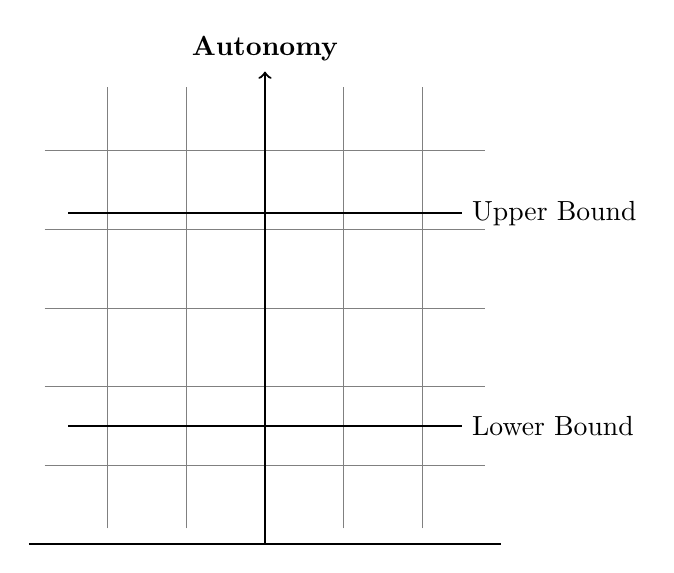
\begin{tikzpicture}
	\draw[step=1cm,gray,very thin] (0.2,0.2) grid (5.8,5.8);
	\draw[thick,-] (0,0) -- (6,0);
	\draw[thick,-] (0.5,4.2) -- (5.5,4.2) node[anchor=west] {Upper Bound};
	\draw[thick,-] (0.5,1.5) -- (5.5,1.5) node[anchor=west] {Lower Bound};
	\draw[thick,->] (3,0) -- (3,6) node[anchor=south] {\textbf{Autonomy}};
\end{tikzpicture}
\\

Sparrow also says that the upper and lower boundaries of this space are fuzzy
CITE. Using this picture, we will later see, how the different authors respond
to the responsibility gap, by placing the upper and lower bounds at different
heights.

On the one hand,
the system is too autonomous for humans to be responsible, on the other hand it
m

%MAKE PARAGRAPH MORE FLOWY


Before moving on, I shall present a brief argument, that will help us structure
the assessment of the question:

The debate around the responsibility gap is centered around the argument that
when an autonomous AI does something, neither the programmer nor the user can
reasonably be considered morally responsible. If then, the AI cannot be
considered responsible as well, we are faced with a sitiuation where something
has happened and no one can be considered responsible. I would like to now go
back and lay out the arguments of those who say that the problem exists in the
first place; those who say that we will not be able to deal with the problem of
responsibility ascription in the same way we are used to by subscribing to the
above mentioned instrumental theory; those who say that the involved humabns are
not responsible nor is the machine. 

%MY ARGUMENTATION MUST BE CLEAR HERE. DO PEOPLE UNDERSTAND WHAT I AM GOING TO?
%WHAT AM I GOING TO IN THE ABOVE PARAGRAPH: THE QUESTION ABOUT THE QUESTION
%ITSELF. WHAT MOTVIATES US TO THINK OF THE RG: HUMANS ARE NOT RESPONSIBLE IN THE
%SAME WAY THEY USED TO BE. LET US EXAMINE WHO SAYS THAT.

\subsection{Why humans cannot be responsible}

Let us reconsider Matthias' argument for the responsibility gap. Matthias says
that\\

\say{[f]or a person to be \textit{rightly} held responsible, that is, in
accordance with our sense of justice, she must have \textit{control} over her
behaviour and the resulting consequences ``in a suitable sense'' (Fischer and
Ravizza 1998:13)}\footnote{According to Matthias this quote can be found in:\\
J.M. Fischer and M.S.J. \textit{Ravizza Responsibility and Control. A Theory of
Moral Responsibility}. Cambridge University Press, Cambridge, 1998.}

Further, he says that machine learning technology will lead to a decrease of
control humans will have over machines and their doings. People will not be able
to predict what a machine does nor understand why it did it. The control
requirement would not be fulfilled and no person could `rightly' be held
responsible.

Matthias does not really consider the machine to be an appropriate locus of
responsibility. I assume that the machines he talks about are just that:
machines, tools, systems to be used by humans. They cannot have
responsibility.\\

Sparrow considers how humans could be responsible and comes to the conclusion,
that, if the system is truly autonomous, no human can be responsible for it. The
programmer could be considered only responsible, if the mistakes the machine
made came as a result of the programmer's negligence. However, Sparrow goes on,
if the possibility of a mistake, say an autonomous weapon system kills the wrong
target, a medical software misdiagnoses a patient, is clearly stated and
disclosed as a \say{limitation of the system} (\cite[p. 69]{sparrow2007killer}),
the programmer is released from bearing the responsibility and it would be taken
over by the user, the commanding officer, the physician employing the
technology. But they as well would not be appropriate targets of responsibility
in Sparrow's view. He reasons that if the AI was truly autonomous, it would
\textit{choose} its actions on its own (\cite[p. 70]{sparrow2007killer}). It
seems to me that Sparrow suggests that an autonomous AI would exercise a will.
And it would not be fair to hold the user responsible for something that
originated from the will of such a machine.

I want to point out that Matthias and Sparrow seem to disagree about the degree of
autonomy a machines would need to have, such that a gap in responsibility
emerges. According to Matthias, the gap will exist pretty much any kind of
machine learning technology, that has the capcity to learn and change its
behaviour and be unpredictable for humans. He specifically mentions neural
networks, genetic algorithms and reinforcement learning; technologies that
already exist. Sparrow talks about systems that are much more sophisticated and
further down the road. For him, the problem of the responsibility gap only
arises with \say{true} autonomy in a philosphically most rigorous sense (see p.
\pageref{sparrow_autonomy}).

'However, legal questions regarding how is responsible for the acrions of
(ro)bot, and when it might cross the threshold to where it bears resposnibility
for its own actions are certainly related to the themes of this book.' -Moral
Machines p.191

%In taking the
%claim of 

%IF THE GAP PERSISTS, IT IS ARGUED THAT WE SHOULD CEASE THE DEVELOPMENT OF SUCH
%AUTONOMOUS ROBOTS (SPARROW/Robots should be slaves etc.). THERE IS ALSO AN
%ARGUMENT TO BE MADE THAT WE AS A SOCIETY TAKE THE RISK OF HAVING THEM BECAUSE OF
%THE BENEFITS THEY PRESENT (Hellström)

%~~~~~~~~~~~~~~~~~~~~~

%I think that, what irritates us, what motivates us to speak of a responsibility
%gap, is the introduction of autonomous machines as

%I shall structure my examination of the three

%QUESTIONS: 
%1) WHAT IS THE AUTHORS MAIN POINT??\\
%2) WHAT KIND OF AUTONOMOUS SYSTEM ARE THEY TALKING ABOUT??\\
%3) WHAT IS THEIR VIEW ON MORAL RESPONSIBILITY??\\
%4) WHO SUPPORTS THEIR ARGUMENT??\\
%5) WHO DISAGREES WITH THEIR ARGUMENT??\\

\subsection{Can Machines Be Responsible?}

If the argumentation above is convincing, there is a degree of autonomy that
machines can achieve that which would render it unfair to hold the programmers and users
responible for it. It then makes sense to explore the third possible locus of
responsibility, that Sparrow talks about: The machine *ominous music starts
playing*

In the discussion about whether machines can be responsible, we find the
sometimes explicit (\cite[p.  489]{SmithVickers2021}), but mostly implicit
assumption that a morally responsible agent is a full moral agent. They are
the same thing. This is in line with Strawsons statement that having reactive
attitudes towards someone is to see them as a member of the moral community
(see page \pageref{responsibility_implies_agency}). Demonstrating the truth of
that assumption goes beyond the scope of this thesis, but I will accept it
because of its intuitive validity. We will thus see that the search for how
machines can be responsible will lead us occasionally to the question about
how machines can be moral agents. So please do not be confused.\\
So, we find agreement among the authors that in order to be responsible,
machines must be moral agents. However, we will encounter a lot of disagreement
about what makes a machine a moral agent or whether they can achieve this status
at all.
Though we find agreement that in order to be responsible, machines must be full
moral agents, we will encounter a lot of disagreement about what makes a machine
a moral agent or whether they can achieve this status at all.

%We will see that most authors agree that a machine can only be responsible, if
%it is a full moral agent. This is in line with Strawsons statement that having
%reactive attitudes towards someone is also to see them as a member of the moral
%community (see page \pageref{responsibility_implies_agency}). bla bla bla make
%it coherent please...
%
%Thus the only
%thing we need to do to explore the possibility of machine responsibility is to
%find out what would make machines moral agents.
%However, they do disagree about what makes a full moral agent a full moral
%agent. Some even say that machines by their nature can never be full moral agents.
%Arguably, if machines cannot be responsible, we do not need to divert from 
%instrumentalism and deal with the stuff just like we have dealt with it in the
%past.

%In light of this, the question of can machines be responsible can be answered in four different
%ways: 

The basic positions regarding the question about machine responsibility can be
summarised in four different ways: Yes, No, Maybe and Kinda.
%\newpage

\subsubsection{How Machines Could Be Responsible}
Who says that and why?

%\textbf{Sparrow: Machines, how ever autonomous they are, cannot suffer, thus they cannot
%properly be held responsible.}\\
Sparrow talks in his essay 'Killer Robots' about Autonomous Weapon Systems, but the
points he makes about moral responsibility are not specific to that particular
domain and are, thus, generalisable. Sparrow acknowledges that a machine
can be causally responsible for some action, but denies that this is enough to
be morally responsible. To be morally responsible is to be open to moral appraisal
(blame or praise) and as a result to be treated accordingly (punished or
rewarded). Sparrow then proceeds imagining how punishing an autonomous machine
might look like. He suggests that a sufficiently intelligent (and therefore
autonomous) machine would probably have internal states akin to human internal
states, that can be described as desires and needs. Punishemnt could
theoretically be done by preventing these desires and needs from fulfillment: If
they earn wages, machines could be fined; their liberty could be restricted by
imprisoning them; or, in the most severe case, they could be destroyed as a form
of capital punishment. However, Sparrow assumes that punishment is only
punishment if the target suffers as a result. And that is a very demanding
condition. It would not be enough, he says, that the machine would suffer
`functionally'. To fulfill our moral demands, the machine's suffering ought to
have a phenomenological quality to it. Otherwise punishing an autonomous system
would be no different from punishing a hammer\footnote{Coeckelberg makes a
similar comparison with a hammer.ZITIEREN}. It wouldn't \textit{really} care.
This means that, according to Sparrow, automonous machines could potetially be
responsible, but only if they have the necessary phenomenology with the
capability to suffer when punished and, consequently, to feel pleasure when
rewarded. Sparrows argumentation seems to rely strongly on a property view of moral
responsibility: To be morally responsible requires the phenomenological
capability to suffer. When it comes to how we could establish whether the
machine had such a capability or not, against my expectations, Sparrow says that
all the machine had to do is to convince us that it had it and evoke appropriate
responses within us humans through its behaviour. This approach heavily
resembles a process view on phenomenological experience. In that case the
machines would be \say{full `moral persons'} with moral rights and duties and
appropriate subjects for moral considerations, that are hitherto reserved for
human beings. MAYBE I SHOULD TAKE OUT THIS LAST HALF SENTENCE (NO SOURCE) (NOT
SELF-EVIDENT)

%PUT HERE A PARAGRAPH ABOUT THE CONCEPTUAL SPACE THAT SPARROW TALKS ABOUT.

%I THINK I SHOULD PUT THE PAPER ABOUT STATISTICALLY RESPONSIBLE AI HERE; THEY
%COME TO THE SAME CONCLUSION; BUT THEIR VIEWS ON MR AND CONSCIOUSNESS ARE
%DIAMETRICALLY OPPOSED. WHICH IS FUNNY.

%PUT CONCLUSION ABOUT THE TWO PAPERS AT THE END OF BOTH OF THEIR DISCUSSION!
%\textbf{Smith/Vickers: Machines can only be responsible, if they are conscious and their
%morality is similar to ours}

Smith and Vickers take a Strawsonian view on moral responsibility, instead.
Additionally they stipulate that in order for machines to be morally responsible
agents their moral system must \say{cohere with the system that we already
have}. This means that it is not feasable to invent a specific machine morality
and marry it with the already existing human morality. That would lead to a
state where ascriptions of responsibility are not understood by every member of
the new moral community and, hence, would not find acceptance. Thus, all members
of the moral community must have the same type of morality. Since we already
have a human moral community\footnote{I use the term human moral community in
	the loosest possible sense, to denote that, in general, most humans
	regard each other as moral beings with the capacity to take
responsibility for their actions.}, the question becomes: Under which
circumstances can an AI become a member of the human moral community? Or in
other words, which capacities must an entity have to be part of our moral
community?

%I THINKT THIS ABOVE IS A GOOD PARAGRAPH 


%Moreover, since we
%are exploring ways for machines to be moral and responsible, by the argument I have just
%presented and the fact, that we already have an established human moral
%community, responsible machines would be fully incorporated into the human moral
%community. For a machine to be moral would have to mean the same thing as for a
%human to be moral. For a machine to be responsible would have to be meaningful
%in the same way as for a human to be responsible. What would it be, then, that
%would make a machine a compelling moral and respoponsible agent, who would be
%part of our moral community?
%
%What are then the
%requirements to be regarded as a member of our moral community?
%
Smith and Vickers argue that there are three core capacities that must be
possessed by every \say{full member} of any moral community (on a Strawsonian
account):


\begin{itemize}
	\item The capacity to have reactive attitudes.
	\item The capacity to recognise other's reactive attitudes as demands
		for a certain type of treatment or regard.
	\item The capacity to respond to reactive attitudes. CITE
\end{itemize}
Thus, we can write on our little list of demands that an AI should have these
capacities.

On top of that, each moral community forms moral traditions and practices that
depend on the specific properties of its members. Based on these properties, we
judge which expecatations, demands and reactive attitudes are fair to have and
which not.

\begin{example}
		We might say that it is morally wrong to drink and drive because
		of all the risks that it bears. But, we can easily imagine an
		animal akin to the homo sapiens with the only differnce that it
		naturally behaves as if drunk. With lower inhibition and motor
		control and worse memory forming capacities. All else being
		eqaul, it seems plausible that a society of these homo
		alcoholicus would form moral
		practices that account for this natural state of its members.
		(CITE HIERONYMI p.31-32)
\end{example}

We see that the moral system that we have developed is a contingent possibility
based on reactive attitudes \textit{and} the expectations that we have based on
certain properties of the population. Moreover, these properties
receive their relevance from their, somewhat, statistical normality and
oridinariness (CITE STAWSON, HIERONYMI, SMITH/VICKERS). 

Any responsible AI would need to have those statistically ordinary capacities.
Smith and Vickers give only few examples of what these ordinary capacities are.
However, they say two things: An AI that has these capacities would act
\say{indistinguishably from us} \textit{and} it would have a will. 
By the author's definition, an AI that behaves like humans and has a will is
called a strong AI and a strong AI is a responsible AI. 

Strong AI stands in contrast to weak AI, which is also indistinguishable from
humans in its behaviour \textit{but} has no will, no inner life. For Smith and
Vickers, having a will is such a fundamental statistically ordinary capacity in
the human moral community, that nothing that does not have a will cannot be
reasonably considered a morally responsible agent.
% It would be exempt from being
% held responsible on the basis of not having that capacity.

Weak AI, however capable, is a mere object and expressing reactive attitudes
towards it, would be no different than expressing them towards a chair. Smith
and Vickers even go sofar to say that it would not be `right'.\\

\say{There is
	something \textit{wrong} with a person who genuinely blames a table when
	they bang their knee, or genuinely blames a baby who throws food. We
might be irritated [...], but \textit{blame} is misplaced.}\footnote{Italics
taken from the original text} (\cite[p. 4-5]{SmithVickers2021}).\\

The authors,
then, see no one who could reasonably be held responsible for such an AI's doings
and we would face a responsibility gap.\\

We can observe that Smith and Vickers come to a similar conclusion as Sparrow:
For an autonomous system to be morally responsible it must have an inner life,
some sort of phenomenology, that legitimises it being a moral agent and not just
a thing. If that is not given, the authors of both papers say that the
responsibility gap persists and it is unclear who should have the responsibility
for what the system does. They conclude that either the AI is responsible on the
basis of having an inner life or nobody is an appropriate object of moral
responsibility.

Notably, Sparrow and Smith/Vickers come to the same conclusion, by taking
diametrically opposed stances on the concept of moral responsibility. It seems
that Sparrow takes rather a property view on moral responsibility. He has a
sense in which someone truly \textit{is} responsible for their actions. Smith
and Vickers, on the other hand, explicitly refer to the Strawsonian take on
moral responsibility, which is a process view on the matter. However, their
requirement for an inner life, in my opinion, does not cohere with the main point
of Strawson's account. In having this requirement they tie moral responsibility
to a metaphysical property that we cannot prove\footnote{Yet?}. That is the very
issue which motivated Strawson to develop his view in the first place. His whole
idea revolves around the point that our moral practices work independent of any
metaphysical properties like freedom of will and intentionality and
consciousness. They instead rely on the interpersonal attitudes we have towards
one another. Imposing the requirement of a will, undoes Strawsons whole
work\footnote{In my humble opinion...}


%END?


% But wasn't that like Strawsons
% whole deal, that he was like, we don't need any of that shit. It's like:
% duuuuude, c'mon!
% 
% I would like to pay short attention to that statement: \textit{In order to rightfully
% be held responsible one must possess a will.} I see it hugely problematic,
% because it seems to miss the main point of Strawson's approach to moral
% responsibility. Strawson's main point was to show that our moral practices work
% independent of any unknown metaphysical properties like freedom of will and
% intentionality and consciousness. They instead rely on the interpersonal
% attitudes we have towards one another. In that sense there is no basis for the
% word `rightfully' to mean anything beyond being accepted in the moral community
% as a norm. Again, the words \textit{to rightfully be held responsible} only make
% sense in the context of the human moral community. I don't think that Strawson
% provides an argument for a cosmic, metaphysical sense of `right'. On the
% contrary, he argues that for our moral practices it does not matter. It then
% seems like a magic trick, how Smith and Vickers define what it means for someone
% to be rightfully held responsible by necessitating a will, an inner life, a
% metaphysical property, that we don't know how to prove. This is something that
% the authors appreciate themselves. Their solution to that is quite vague and
% resembles the one Sparrow has: We say that an AI has inner life, if it behaves
% in a way that leaves no doubt about it.
% 
% 
% 
% What, then, is needed for a machine, an AI, an autonomous system, call it
% whatever you like, to become a full member of the moral society? Well, it needs
% the 3 core capacities to 
% 
% 
% 
% Referring to Pamela
% Hieronymi's analysis of 'Freedom and Resentment', the authors admit
% that on a Strawsonian account different variations of moral communities are
% concievable (CITATTION). The morality, that we have developed is a contigent
% possibility based on reactive attitudes \textit{and} our general and
% statistically ordinary capabilities. These statistically ordinary capabilities
% are a heuristic that we use to determine what is fair to expect. If people by
% nature behaved as if drunk, with lower inhibition and motor controll, it seems
% very plausible, that we would be expecting different things of one another and would
% thus have had developed a different moral framework that accounts for how people
% generally are.
% 
% However, the moral community, we are interested in is the human
% one. AI must perform well on an intuitive and human account of moral
% responsiblity in order to be compelling moral agents from a human perspective.
% 
% Smith and Vickers argue that the human members of the moral community have certain properies that
% we hold necessary to be a member of that community\footnote{Being a member of the moral
% community is per definition also being a moral agent and being regarded as such.}
% 
% 
% Smith and Vickers come to a very similar conclusion. Curiously, though, through
% an approach that is diametrically opposed to Sparrow's. While Sparrow takes a
% property view on responsibility and puts a condition of process view phenomenological
% consciousness, Smith and Vickers take a Strawsonian approach to moral
% responsibility (which as we explored earlier comes from a process view), but
% condition it with metaphysical properties like empathy and will. Their argument
% goes like this: In order for machines to be morally responsible, they must
% become members of the existing moral community. Inventing a new type of morality
% specifically for machines and then marrying the existing and new morality
% together would not work, because that would mean that the morality of some
% members of the new moral community would not be intelligible and intuitive to
% other members. Such a community would not find any acceptance. Thus, all members
% must have the same type of morality. To be a member of the currently existing
% moral community, one must be an appropriate target for reactive attitudes
% (taking the Strasawnian approach). For the authors, being an appropriate target
% means that the individual must have certain core capacities:
% \begin{itemize}
% 	\item The capacity to have reactive attitudes.
% 	\item The capacity to recognise other's reactive attitudes as demands
% 		for a certain type of treatment or regard.
% 	\item The capacity to respond to reactive attitudes.
% \end{itemize}
% 
% I would like to, again, draw attention to the word `appropriate' (the authors
% also use `rightful' in the same context). For Strawson the appropriatness of
% reactive attitudes is in a sense negotiated between the source and the object.
% Smith and Vickers, citing Hieronymi statistically ordinary capacities. While I
% think that Strawson might agree, that certain conditions for the perceived
% appropriatness of reactive attitudes can be nailed down by their statistical
% prevalence, their metaphysical significance does not matter for reactive
% attitudes.
% 
% Machines can be responsible if they are appropriate targets for
% reactive attitudes.
% 
% THey do not talk about how moral norms can change with changes in the society. I
% found source for that in exactly hieranymi Chapter 2 page 25-26!!!
% https://www.degruyter.com/document/doi/10.1515/9780691200972/html?lang=de
% It is kind of implied but never discussed with the depth it seems to deserve.

At this point we have considered two positions that both come to the same
conclusion: Robots, AI, autonomous systems can be responsible, but only under
the condition that they have some sort of phenomenology, will or inner life. As long
as that is not given, we face a responsibility gap.

%Two questions come to mind. First: Can we perhaps still imagine an AI that does
%not have the demanded qualities but can still be considered responsible. Second:
%Is it true that we face a responsibility gap, if the machine cannot be
%responsible? What about the other involved players?
%IS THE SECOND QUESTION FAIR? PERHAPS IT IS TOO BIG? PERHAPs TAKE OUT THE WHOLE
%PARAGRAPH? IT IS NICE BUT ONLY IF I FIND A MORE RIGOROUS QUESTION.

A question immedeatly comes to mind: Can we perhaps still imagine an AI that
does not have the demanded qualities but can be considered responsible anyway?

John P. Sullins, for examplem, is not as demanding when it comes to moral responsibility. 
He writes that a robot can be responsible, if ascribing responsiblity to it
is the best way to explain its behaviour. This is a process view on
responsibility. For Sullins assuming responsibility
comes from a `belief' of duty to do something. This belief must not originate
from something we might call consciousness or a thought. This is probably the main
difference between what Sullins thinks and what Sparrow and Smith/Vickers think.
As he cynically remarks: \say{The machine may have no claim to consciousness,
[...], or any of the other somewhat philosophically dubious entities we ascribe
to human specialness}(\cite[p. 159]{sullins2006robot}).To Sullins, `belief' is a
functional term to describe something that motivates one to solve moral problems
in a certain way (\cite[p. 159]{sullins2006robot}).
PUT THIS IN A LATER SECTION ?:
Machines that are not regarded as responsible agents can still be moral entities
if they have sufficient autonomy and intentionality. Just like responsibility,
these attributes can be merely apparent. Such machines should be targets of
moral considerations. Sullins suspects that their moral status will be similar
to the status that for example dogs have and their owners are the ones who are
responsible for them(\cite[p. 159]{sullins2006robot}).\\
Here, Sullins does not leave room for a responsibility gap. He says that the
user assumes the responsibility for an autonomous system until it fulfills the
requirements to be responsible on its own. As I already said, these requirements
are not very strict compared to Sparrow and Smith/Vickers. A machine's moral
status is dependent on its role in society and how it is regarded by the
society; further properties, such as consciousness, are secondary or even
irrelevant.

We find two statements here, that are relevant for the topic at hand. Firstly,
Sullins grants that machines can be responsible, if it makes sense to describe
their behaviour in such a way. Secondly, he says that if
machines are not responsible, the humans behind the machines are. There is no
conceptual space for the responsibility gap. Still, there is a somewhat clear
boundary for what makes an agent responsible.

%MAKE A NICE TRANSITION TO COECKELBERGS PAPER.

Sullins' position is supported by Mark Coeckelberghs argumentation about the
moral standing of machines.

That boundary entirely falls away in Coeckelbergh (\cite{coeckelbergh2014moral}).

According to Mark Coeckelberg, there is a mismatch between how we usually think
about machines in general and how we \textit{sometimes} act towards them
(\cite[p. 61]{coeckelbergh2014moral}). We tend to think of machines as
things and tools that do not have any kind of moral standing. To have a certain
kind of moral standing an entity must have a certain property, or a set of
certain properties. This is clearly a property view; Coeckelbergh calls it \textit{the
standard approach} (\cite[p. 62]{coeckelbergh2014moral}). These properties could be the
usual suspects: Consciousness, the capacity to suffer, etc. (\cite[p.
62-63]{coeckelbergh2014moral}). And machines just do not seem to have these
properties, that is why people are reluctant to give them the status of a full
moral agent.\\
According to Coeckelbergh, there are several problems with this
view. First of all there are epistemological issues. We have no way of
objectively observing the relevant properties; there is also no objective way to
bind a specific moral status to a specific property
(\cite[p. 63]{coeckelbergh2014moral}). Furthermore, there is a
cleft\footnote{Coeckelberg actually calls it a \say{gap}, but for obvious reasons I
decided to alter his terminology.} between the just described way we think about
machines in general and how we treat them. Coeckelbergh says that we
sometimes ascribe emotions, personalities and \say{presence} to them (\cite[p.
62, 64]{coeckelbergh2014moral}). We may care about them and develop
relationships with them. From the perspective of the standard approach this
behaviour would be not \say{correct} or rational (\cite[p.
64]{coeckelbergh2014moral}). These problems are sufficient for Coeckelbergh to
question the standard approach.\\
 Thus, he introduces \textit{the relational approach} to how we assign
moral status and, with it, responsibility. This account is a process view and it
emphasises the relations the entity in question has with other entities. And
\say{moral status [is] something that emerges through relations between
entities} (\cite[p. 64]{coeckelbergh2014moral}). Moreover, the relation that
matters most is the relation between the entity itself and the one who ascribes
the moral status to it. Whether a particular machine is an appropriate object of
moral considerations, whether it can hold responsibility is for the observer to
decide. It is a highly subjective decision that strongly depends on the relation
they have with the machine.This implies that moral status is not only not
objective, but it is also not universal. On this view, there is no correct way
to view an autonomous system and different people would judge differently.\\
Note that Coeckelberghs account is much more permissive compared to everything
else that we have encountered. Using the Strawsonian terminology: If the
relation to an entity is such that one develops reactive attitudes towards it,
one regards it as a responsible moral agent, regardless of what the entity in
question is. Other authors pose specific requirements to establish which
entities are `appropriate' targets of reactive attitudes and which are not.
Smith and Vickers argue that it is only appropriate, if the target has an inner
life. Sullins says that it is legitimate to have reactive attitudes towards a
machine, when its behavioural complexity matches the the human one and it is
`reasonable' to assign agancy to the machine in view of its behaviour
(\cite[p. 169]{sullins2006robot}). All of these and other requirements fall away
with Coeckelberghs relational approach. There is no such thing as an
`appropriate target' of reactive attitudes. This, of course, means that we do not
stop at intelligent machines regarding the question of moral standing. Other
types of entities can have moral standing.

\begin{example}
	In early 2020, I visited the Wellcome Collection in London. One of
	the vitrines diplayed several masks, that were collected from different
	indigenous tribes from all over the world. One of the spots was empty.
	The guide explained that the tribe where that mask was taken from, has
	demanded it back. These masks were inhabited by the ghosts of deceased tribe
	members and they regarded and treated them as real people.
\end{example}

Under the standard approach\footnote{Caveats may apply: We are situated in the
western culture, etc.}, viewing the mask as a person does not really make
sense. We might say that the tribes care for the mask comes from a believe
rooted in tradition, religion and culture, but the mask is a mere thing without
an objective moral status. Coeckelberghs relational approach on the other hand,
allows for \say{multisubjectivity and plurality of truths} (\cite[p.
66]{coeckelbergh2014moral}). Coeckelbergh argues that this view treats morality
not as an abstract philosophical concept, but accords with the reality of human
everyday life and asks the question of moral standing on an individual basis (\cite[p.
66]{coeckelbergh2014moral}). It respects how a particular entity is situated in
personal, social, cultural, natural and other contexts.\\

%HERE I MUST PUT SOME KIND OF CONCLUSION. OTHERWISE THE WHOLE THING JUST ENDS.
%SOMETHING LIKE:
This seems like a very extreme approach and demands a reevaluation of the way we
conceptualise moral agency and responsibility. BLABLA BLA

Daniel Tigard takes a slightly different path. His account of moral
responsibility leaves the question whether it is a process or a property
view unanswered. However, Tigard subscribes to a pluralistic account of
responsiblity (\cite[p. 442-444]{tigard2021artificial}). This means that there
are different ways in which agents can be considered responsible. For example,
agents are responsible for their characters in a different way than they are
responsible for their evaluative judgements\footnote{See (\cite{Shoemaker_2011})
for further information}. According to Tigard, such pluralistic approaches are
very flexible and expandable (\cite[p. 442-444]{tigard2021artificial}). He
proposes that as autonomous systems become more ubiquitous and the question of
responsibility becomes more relevant, we might develop additional conceptions of
what responsibility is that fit into this pluralistic view. He does not claim, that
machines will be responsible in the very same sense as humans. Instead, there
will be another conception of responsiblity, an artificial responsiblity that
can only target artificial moral agents. In that, Tigard disagrees with Smith
and Vickers about their claim, that machine responsiblity must be the same as
human responsiblity. He also disagrees with Sparrows point that in order for a
machine to be responsible it must be punishable - and for it to be punishable,
it must have the capacity to suffer.  This is a retributivist account of
punishment (\cite[p. 77]{sparrow2007killer}, \cite[p.
441]{tigard2021artificial}). According to Tigard, there are alternative
conceptions to punishment and they do not necessarily require the suffering
part. Punishment can also be seen as a rehabilitation with the aim to achieve
certain changes in the target and help it imporove (\cite[p.
442]{tigard2021artificial}). Now, it is possible to punish a machine in that
sense, by restricting it in certain ways or changing its code or what ever one
can come up with (\cite[p. 443]{tigard2021artificial}). Suddenly, Sparrows
argumentation of why machines cannot be responsible falls away, because
responsiblity, under this approach, does not rely on an inner life or similar
things.\\
To summarise, Tigard proposes that there is no reason that machines must
necessarily be responsible in the very same way as humans. Referring to a
pluralistic approach of moral responsibility, he explores what it would mean to
have sort of an artificial moral responsibility that could be applied to
powerful AIs.\\

In this section, we have discussed what makes an autonomous system responsible.
We have seen a gradual decline in what machines need to be in order to be
responsible for their actions.\\
Sparrow and Smith/Vickers claim that in order for them to be responsible, AIs
must have an inner life in the strongest possible sense. Otherwise all
attributions of responsiblity would be misplaced.\\
Sullins' position is less rigid and proposes a rather functional account of
responsibility. To him, machines can be regarded as responsible agents as soon
as doing so is a sensible and natural way to explain their behaviour.\\
Coeckelbergh recognises that there is a mismatch between how we think about
moral agency and responsibility and how we actually ascribe them. He further
explains that there are epistemological problems with how we traditionally
conceptualise the matter by looking at the properties of the entity in question.
Instead, he explores the possibility that moral status is ascribed on the basis
of the relation between the entity itself and the one who ascribes the moral
status. In that sense, responsibility is something that is only ascibed by the
observer and has no underlying universality to it.\\
Tigard relies on the pluralism of responsibility and says that we might
expand our current notions by developing some sort of artificial responsibility.\\



%This, Coeckelbergh says, allows for 
%
%Sullins says that 
%
%they will be targets of moral
%consideration. Sullins suspects that they will then 
%WRITE ABOUT
%SMITH ANS VICKERS OBJECTION



%Sullins
%proposes, that machines can be regarded as responsible agents, if they act as
%such (\cite[p. 159]{sullins2006robot}). This sounds very similar to what Sparrow
%and Smith/Vickers say. However, while the previous authors put a requirement on
%an inner life, Sullins does not. For Sullins the machine is responsible, if its
%behaviour can only be explained by attributing responsibility to it. No will,
%consciousness, or phenomenology necessary.\\
%What does it mean then for Sullins to behave \say{in such a way that we can only
%	make sense of that behavior by assuming [the machine] has has
%responsibility to some other moral agent(s)} (\cite[p. 159]{sullins2006robot})?


%PLACE TIGARD HERE AND SULLINS AND COECKELBERG

%\textbf{Johnson: Machines cannot be full moral agents bla bla, I am not sure what she
%says}
%\textbf{Bryson: Robots should be slaves. Otherwise we will use them to evade
%responsibility}
%\textbf{Marino/Tamburrini: Implicit neglection of the option}
%\textbf{Champagne/Tokens: Implicit neglection of the option}


\subsubsection{Why Machines Cannot Be Responsible}
%Discuss artificial agency
%\textbf{Tigard: different types of responsibility/SmithVickers would probably
%disagree, because the machines would have a different morality than humans and
%that is not morality}
%\textbf{Coeckelberg: It all depends on what position in society they will have.}
%
%\textbf{Sullins: Robots can be functionally responsible. If the only way to make sense
%of a robots behaviour is to ascribe some responsibility to it, then it is
%responsible.}

%Sullins approach is a bit different insofar as he says that being able to be
%responsible is a precondition for the machine to be an autonomous agent, not the
%other way around. 

In a sense, the positions from the previous section all advocate for leaving behind
the instrumentalist theory of technology. As a reminder, the instrumentalist theory
supposes that computers and machines and all their derivatives are tools
that are constructed with a human goal in mind and do not have their own ends
(\cite[p. 308]{gunkel2020mind}). It follows that the responsibility for any
action that originates in this technology should be ascribed to the relevant
humans. The arguments from the last section invite us to abandon this 
theory by either permitting the (at least conceptual) possibility of technology
that is not a tool, but a moral agent with its own goals - or denying that
responsibility necessarily falls onto those who set the ultimate ends.
Naturally, there are voices that hold on to the instrumentalist theory and doubt
that machines can (or should) ever be responsible agents. Let us explore what
they have to say.

One way to argue against machines being proper responsible agents is of course to
point to a theory of moral responsibility and explain why they are not eligible
for being considered as such. For example, we might remember Smiths account of
moral responsibility (see page \pageref{smith}). Agents are responsible for
those and only those actions that are based on evaluative judgements. Can
machines have evaluative judgements?
SHOULD I PUT IN THIS PARAGRAPH?

\newpage
Deborah Johnson is one of these voices (\cite{johnson2006computer}). She argues
that no man-made artifact can ever be a moral agent on its own. Her postion rests on, what
she calls, the \textit{standard account of moral agency and action} (\cite[p.
198]{johnson2006computer}). In order for an action to be open for moral
evaluation, it must meet five conditions (\cite[p.
198]{johnson2006computer}):

\begin{enumerate}
	\item The agent must have internal mental states (such as desires,
		beliefs, wishes) that motivate a behaviour. One of these states
		is an intending to act. Without that, there would not be an
		action. Johnson says that these internal states are the
		\textit{reasons} for an action (\cite[p.  198]{johnson2006computer}).
	\item Something happens. There is an external and embodied behaviour.
	\item The behaviour is caused by the agents internal states as a
		rational means to accomplish their end.
	\item The behaviour causes an outward effect.
	\item The effect acts on a moral patient, an entity that is subject to
		moral considerations.
\end{enumerate}

Only when an entity is capable of performing these kinds of actions, it can be
considered a moral agent. We see that this is a property view on moral agency.\\

Johnson says that computers can easily fulfill the conditions 2,3,4 and 5. The
second condition is met by computers being able to portray a behaviour by
changing the screen and audio output or moving physical parts by controlling a
motor. Since this behaviour is regulated by the machines internal states, the
third condition can be checked off. That the behaviour can have effects on the
outside world and act upon moral patients is obvious and these are exactly the
conditions 4 and 5.\\
Condition 1 is trickier though. It states that the internal states of an agent
are mental states and that one of these states is the intending to act. Johnson
focuses on the second part and claims that computer systems will never have a
true intending to act. The intending to act, so Johnsons reasoning, comes from
an agents freedom. \say{Action is the exercise of freedom and freedom is what
makes morality possible} (\cite[p. 198]{johnson2006computer}). Thus, if an
entity is not free in that sense, it cannot act and is not an agent. Human
behaviour has non-deterministic component to it, that \say{mysterious[ly]} makes
the freedom (\cite[p. 198]{johnson2006computer}). One could now argue, that if
computers have the ability to learn, their behaviour will also be
non-deterministic. However, the way in which humans are undetermined is
different for the way machines are; or at least it is unclear how to compare the
two ways (\cite[p. 198]{johnson2006computer}). From this, Johnson concludes that
Machines do not have the relevant type of freedom and consequently cannot
develop intendings to act. Condition 1 in not met, computers cannot be moral
agents.\\
Further, Johnsons says that machines have intentionality, but this
intentionality is put into them by their designer and user. The machines
intentionality can be captured by their functionality and it allows it to behave
autonomously. Still, the functionality is determined by the designers and users
goals.\\
This view of autonomous systems is loyal to Heideggers instrumentalist theory
and the responsibility falls onto the humans as the agents that use these
systems as tools.
In short, machines are not moral agents and cannot be responsible for their
actions because they do not have the necessary intendings to act. Their
functionality is determined by the goals of those humans that design and use
them. Therfore, they are responsible for the machines.

While I do believe that Johnson holds an important position, that is in line
with a commonplace conception of technology, I find that she fails to
convincingly demonstrate that machines have not intedings to act. She claims that
intendings to act arise from an agents freedom. Humans have freedom because
their character is non-deterministic, that is why they can have intendings to
act. She further says that machines can also behave in a non-deterministic way.
But because of the differences in how humans and robots are composed, we can
never \textit{really} know, whether their non-determinism grants them the same
freedom that humans are so blessed to enjoy. (may enjoy.)\\ It would then be a
mistake to to claim that they can ever have the relevant type of freedom.
Instead she asserts that computers can never have it (\cite[p.
203]{johnson2006computer}). Here we see the jump in Johnsons logic. She
acknowledges an epistemological limitation and concludes that this limitation
implies the metaphysical difference.\\

Johnsons second point is a bit more convincing. In stating that the
intentionality that autonomous systems have is put into them by humans, the
instrumentalist theory binds them together and makes the humans responsible.
They are the ones who determine the goal, the use, the purpose of technology -
not technology itself. I am missing a comment about why this will also never be
a case in the future, why there is no conceptual space for an autonomus system
with its own intentionality and goals.\\

Joanna Bryson also subscribes to the instrumental theory. She says that
\say{[we] determine their goals and behaviour [...] through specifying their
intelligence [...]}(\cite[p. 3]{bryson2010robots}). This makes us humans
responsible for them. She also provides a line of reasoning that
might be taken as an argument against Sullins' and Coeckelberghs positions as
they are described above. Bryson writes that there is a moral cost in accepting
machines as agents, when they are, in fact, not (\cite[p. 2]{bryson2010robots}).
The cost can be found on an individual level and on an institutional level.
Accepting machines as responsible agents would necessarily lead to their
humanisation. They would be treated as peers to humans. People would befriend them and
spend a lot of their \say{social capital} on them (\cite[p.
5]{bryson2010robots})\footnote{Bryson takes the term social capital from
	Putnam:\\
Putnam, Robert D. \textit{Bowling alone: The collapse and revival of American
community.} Simon and Schuster, 2000.}. 
This means, that these people would have less capacity to socialise with other
humans, their actual peers. Bryson suspects that people would actually prefer
interactions with robots, because they would be easier and not as messy as true
human-human interactions. She does concede though, that people who are lonely
anyway would definetely benefit from these artificial interactions(\cite[p.
5]{bryson2010robots}). 


Machines that behave responsibly and human like 

Deborah Johnson says that machines \textit{will} never have their own ends.
Joanna Bryson says that machines \textit{should} never have their own ends
(\cite{bryson2010robots}). In her paper, she writes that robots should remain
subordinates. They should be tools not moral agents. There is a moral cost in
trying to make them agents which, for Bryson, is too high.
Accepting machines as responsible agents would necessarily lead to their
humanisation. They would be treated as peers. People would befriend them and
spend a lot of their \say{social capital} on them. This means, that these people
would have less capacity to socialise with other humans, their actual peers.
Bryson suspects that people would actually prefer interactions with robots,
because they would be easier and not as messy as true human-human interactions 



%if the
%behaviour does not come from an intending to act, it is not an execise of
%freedom and is not a moral action. 
%
%Who are the candidates?: The manufacturer, the user, the machine
%If the machine is responsible does it imply moral agency/ we must develop
%reactive attitudes. -> What are the conditions for developing reactive attitudes
%towars machines (Statistically responsible AI Vickers and Smith)
%Shoemaker has another example about the aliens, that might eb fitting here
%
%Essentially: How do machines fit into these frameworks
%Upper bound - lower bound of moral agents
%
%Yes we can: Here is how
%Instrumentalism 2.0
%	There is a moral risk in using unpredictable machines and the
%	users/manufacturers that use them accept this risk and are (implicitly)
%	accepting the responsibility. Analogy: There is a risk in using medical
%	drugs because of the side effects.
%Machine Ethics
%Hybrid responisibility
%
%No, we cant: Here is why:

\section{Real World Problems}
\subsection{Autonomous Weapon Systems}
\subsection{Healthcare}
\subsection{COMPAS}
\section{Discussion}

I don't speak of the technical side. This is something that is actually really
important, because how the robot actually is, how it is programmed can determine
its moral capacity and how we view it. (Johnson: Technology without any human
responsibiltiy)


We do not pretend to be able to predict the future of AI. Nevertheless, the 
more optimistic scenarios are, to our skeptical minds, based on assumptions 
that border on blind faith. It is far from clear which platforms will be the most 
successful for building advanced forms of AI. Different platforms will pose 
different challenges, and different remedies for those challenges. (Ro)bots 
with emotions, for example, represent a totally different species from (ro)bots 
without emotions. - Moral Machines p.194

War robots are bad? We want the moral cost and risc be very high.

Hypothesis: We could say that machines are capable of being moral and
responsible, if they, if left alone, would develop some sort of morality of
their own. This seems to be an empirical question. I find this very compelling

The authors talk about responsibility for actions and attitudes but there is
very little talk about responisbility for consequences, which seems even more
important in the context of AI.

In some cases we need to decide what our moral obligation is. Is it more moral
to create a system, where no one is really morally responsible, but there are
much less bad outcomes because machines perform better than humans (e.g.
autonomous vehicles) or is it so important that we can find moral responsibility
in such cases that we cannot turn to such a system

Strawson talks about a resource that we all have: We can regard someone with
objective attitudes who we usually regard with a reactive attitude. What if,
then, we have another resource? What if we have the resource to regard somthings
with a reactive attitude that we would usually regard with an objective
attitude? Cite: FREEDOM AND RESENTMENT PAGE 10. ALSO IN HIERONYMI
\section{Conclusion}

CITE COECKELBERGH ENDE 65-66 about philosophy should not try to close the
discussion about moral standing but instead keep it open. It is so good as a
finishing thought!
\section{Meditation}
WHAT IS THIS SECTION ABOUT?
MY THOUGHT ON MY JOURNEY.

I CHANGED MY VIEW ON MORAL RESPONSIBILITY
IT WAS DIFFICULT FOR ME TO AVOID RABBIT HOLES

This topics is insanely chaotic without structure and perbe without even
sufficient legitimacy for the question itself(?).

How to differenciate between normative and descriptive approaches and problems?

My ideas for future research: Would it be a good measure to determine a machines
moral standing by isolating a society of these machines and observe if they
develop something like a morality themselves?

Are some of the proposed approaches against the ideas of the enlightenment?

Talk about the resource but the other way around.
\section{Disclaimers}
Put this in the beginning or even better into the introduction

Blame and praise are asymmetrical in how we pay attentio to them . While it
might be an interesting intellectual execise to think about who deserves credit
for a piece of art produced by a machine learning algorithm the question of
responsiblity seems far more pressing for when an automated car runs over a
pedestrian or a medical software misdiagnoses a patient. I will thus, mostly
restrict my search for responsibility to cases in which we want to blame.
REFERENCE: SMITH BEING RESPONSIBLE VS HOLDING RESPIONSIBLE P.5
\section{Acknowledgements}
\clearpage

\printglossary[type=\acronymtype]
\printglossary
\printbibliography
\end{document}
